\documentclass[10pt,twocolumn,letterpaper]{article}
\usepackage[margin=0.7in,columnsep=0.25in]{geometry}
\usepackage{times}
\usepackage[T1]{fontenc}
\usepackage{graphicx,booktabs,amsmath,multirow,array,xcolor,enumitem}
\usepackage[hidelinks]{hyperref}
\usepackage{caption}
\usepackage{balance}
\captionsetup{font=small,labelfont=bf,skip=3pt}
\setlist{itemsep=0pt,topsep=1pt,parsep=0pt,leftmargin=11pt}
\usepackage{titlesec}
\titlespacing*{\section}{0pt}{5pt}{2pt}
\titlespacing*{\subsection}{0pt}{3pt}{1pt}
\titleformat*{\section}{\normalsize\bfseries}
\titleformat*{\subsection}{\small\bfseries}
\setlength{\textfloatsep}{6pt}
\setlength{\floatsep}{5pt}
\setlength{\dbltextfloatsep}{6pt}
\renewcommand{\arraystretch}{1.02}
\newcommand{\dec}[1]{\par\noindent\textit{Decision:} #1\par}

\title{\vspace{-1.6em}\large\textbf{Phase 1: FIFO Baseline and Calibration for Memory-Aware Scheduling of Multi-Step Agents}\vspace{-1.8em}}
\author{}
\date{}

\begin{document}
\maketitle

\section{Goal and Setup}
The project asks whether a scheduler that anticipates memory demand and agents returning from tool calls can beat FIFO on throughput and task latency under a fixed memory budget. Phase~1 has two deliverables from the proposal: (a)~FIFO with fixed concurrency $N$, tested at several limits to pick the best fixed-concurrency baseline, and (b)~calibration of the request-memory, run-time, tool-return and recompute-cost estimates that Phase~2 needs.

\textbf{System.} One pinned \texttt{llama-server} (llama.cpp b11780) serving Qwen3-0.6B Q8\_0 with f16 KV in a \emph{unified} KV pool (\texttt{-kvu}, \texttt{-np}$=N$), prompt caching on, host cache off. A read-only patch exports physical occupied KV cells. Final runs use an AWS NVIDIA T4. One KV cell costs 112\,KiB, so the 32K-cell pool reserves 3.5\,GiB at startup.
\textbf{Workload.} AgentTrace tasks (MBPP, NL2Bash) replayed as scripted request/tool-wait sequences: greedy decoding, fixed output budgets, \texttt{ignore\_eos}, saved tool delays ($150\times$, capped at 10\,s), and each next prompt $=$ previous prompt $+$ generated tokens $+$ recorded tool result. Request FIFO dispatches the queue head whenever fewer than $N$ requests run; a task frees its slot during tool waits but its cache may stay resident.
\textbf{Metrics.} Completed tasks (failures kept in the denominator), throughput (completed tasks/min), successful-task p50/p95 latency, queue wait, physical KV occupancy, device memory, cache reuse and failure cause.

\section{Smoke Tests and What They Decided}
\textbf{S1 -- Feasibility (10 burst runs).} A fractional L4 (6\,GiB slice) completed only 2--10 of 50 tasks with a 16K pool and 34/50 with 32K at $N{=}8$. On a matched Poisson-40\,s sweep the T4 completed 550/550 task executions vs.\ 468/550 on the L4, with a 23\,s vs.\ 767\,s median at $N{=}2$. T4 device memory stayed flat at 4.4\,GiB because KV is preallocated.
\dec{T4 with a 32K unified pool; any failure is then due to the KV budget, not device memory.}

\textbf{S2 -- Light load (T4, Poisson 40\,s, $N{=}1$--16).} All levels completed 50/50 at near-identical throughput (1.52--1.56/min); at most five requests were ever active. Turning off prompt reuse raised prefill 9.4$\times$ but moved median latency by only 1.5\,s; removing tool delays moved it by 1.0\,s.
\dec{Arrivals must be much faster to distinguish $N$. Generation dominates service time.}

\textbf{S3 -- Instrumented grid ($N\in\{2,4,8,16\}\times$ 3 arrival patterns, 50 tasks).} Table~\ref{tab:s3}. (i) For $N\ge4$ the pool hit 97--100\% occupancy while the GPU stayed at 4{,}383 of 15{,}360\,MiB; all 138 failures were KV-context errors. (ii) Completion depended on $N$, not arrivals, except at $N{=}16$. (iii) Burst $N{=}16$ had the highest throughput (4.80/min) by failing 32 of 50 tasks, so speed must be read with completion. (iv) Poisson runs never reached 16 active requests (max 11/14). (v) Only 32 size-only backfill opportunities appeared, none at $N{=}16$.

\begin{table}[h]
\centering\small
\caption{S3: tasks completed out of 50 (tasks/min), 32K pool.}
\label{tab:s3}
\setlength{\tabcolsep}{4pt}
\begin{tabular}{@{}lcccc@{}}
\toprule
Arrival & $N{=}2$ & $N{=}4$ & $N{=}8$ & $N{=}16$\\
\midrule
Burst & 50 (2.95) & 46 (3.38) & 34 (4.00) & 18 (4.80)\\
Poisson 5\,s & 50 (2.95) & 46 (3.26) & 34 (4.14) & 22 (4.11)\\
Poisson 10\,s & 50 (2.98) & 46 (3.41) & 34 (3.41) & 32 (3.55)\\
\bottomrule
\end{tabular}
\end{table}

\textbf{Gaps left open.} 50 tasks are too few for tail latency or failure rates (N2 vs.\ N4 differ by 4 tasks); $N{=}16$ was never saturated under Poisson; 64K was only tried with 20 tasks; there was no zero-contention reference.
\dec{Scale to 500 tasks and run seven targeted configurations (Table~\ref{tab:design}).}

\section{Full-Run Configurations}
\begin{table}[h]
\centering\small
\caption{Full runs (500 tasks each) and why each was chosen.}
\label{tab:design}
\setlength{\tabcolsep}{2.5pt}
\begin{tabular}{@{}c c c c >{\raggedright\arraybackslash}p{4.15cm}@{}}
\toprule
Run & $N$ & Arrival & KV & Rationale\\
\midrule
R1 & 1 & Pois.\ 10\,s & 32K & Reliability reference: no overlapping contexts; tests whether any single task is infeasible.\\
R2 & 4 & Pois.\ 5\,s & 32K & Primary: best throughput/completion trade-off in S3 (+10--15\% over N2 for 4/50 lost); N8 lost 32\% everywhere.\\
R3 & 16 & Pois.\ 5\,s & 32K & Stress test, same arrivals as R2.\\
R4 & 4 & Pois.\ 2\,s & 32K & Does N4 stay reliable with a deeper queue?\\
R5 & 16 & Pois.\ 2\,s & 32K & Faster arrivals to actually reach 16 active.\\
R6 & 4 & Burst & 32K & Worst-case arrival shape for N4.\\
R7 & 16 & Pois.\ 2\,s & 64K & Separates capacity from concurrency as the cause of N16 failures (ample VRAM headroom).\\
\bottomrule
\end{tabular}
\end{table}
All runs share the model, build, task file (seed~2), saved delays, prompt reuse, a 21{,}600\,s deadline and a 1{,}800\,s request timeout. N8 was dropped (no new regime); N1 replaces N2 as the zero-failure reference because it removes KV contention entirely. \textbf{Expectations from S1--S3:} R1 completes everything; N4 loses a small, arrival-independent fraction; N16 fails most tasks, worse with faster arrivals; 64K helps N16 but does not fix it; all failures are KV-context errors.

\section{Results}
\begin{table*}[t]
\centering\small
\caption{Full-run results, 500 tasks. Latency is over successful tasks only. Peak KV is sampled physical occupancy of the pool.}
\label{tab:full}
\setlength{\tabcolsep}{4.5pt}
\begin{tabular}{@{}cccc rrr rr r r rr@{}}
\toprule
Run & $N$ & Arrival & KV & Done & Failed & Success & p50 (s) & p95 (s) & Tasks/min & Avg running & Peak KV & GPU MiB\\
\midrule
R1 & 1 & Pois.\ 10\,s & 32K & 500 & 0 & 100.0\% & 4{,}029 & 7{,}351 & 2.70 & 1.00 & 49.0\% & 4{,}383\\
R2 & 4 & Pois.\ 5\,s & 32K & 480 & 20 & 96.0\% & 2{,}874 & 4{,}768 & 4.21 & 3.99 & 99.9\% & 4{,}383\\
R3 & 16 & Pois.\ 5\,s & 32K & 177 & 323 & 35.4\% & 24 & 58 & 4.36 & 6.40 & 100.0\% & 4{,}383\\
R4 & 4 & Pois.\ 2\,s & 32K & 472 & 28 & 94.4\% & 3{,}984 & 5{,}420 & 4.26 & 4.00 & 99.9\% & 4{,}383\\
R5 & 16 & Pois.\ 2\,s & 32K & 100 & 400 & 20.0\% & 127 & 270 & 5.55 & 15.72 & 99.9\% & 4{,}377\\
R6 & 4 & Burst & 32K & 476 & 24 & 95.2\% & 4{,}241 & 6{,}050 & 4.30 & 4.00 & 99.9\% & 4{,}383\\
R7 & 16 & Pois.\ 2\,s & 64K & 340 & 160 & 68.0\% & 1{,}959 & 3{,}631 & 4.48 & 15.05 & 100.0\% & 7{,}999\\
\bottomrule
\end{tabular}
\end{table*}

\begin{figure}[t]
\centering
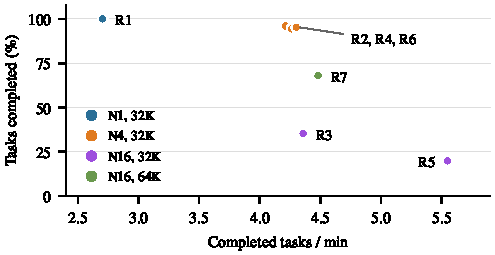
\includegraphics[width=\columnwidth]{fig_tradeoff.pdf}
\caption{Completion vs.\ throughput for the full runs. N4 sits at the knee; N16's higher throughput comes from failing most tasks.}
\label{fig:trade}
\end{figure}
All five expectations held (Table~\ref{tab:full}, Fig.~\ref{fig:trade}).
\begin{itemize}
\item \textbf{KV pool, not VRAM, is the bottleneck.} All 955 failures are KV-context errors; no timeouts. Every $N\ge4$ run filled the pool while using at most 52\% of VRAM.
\item \textbf{No task is infeasible alone.} R1 completed 500/500 with a 49\% peak, so every failure comes from concurrent contexts competing for the pool.
\item \textbf{N4 is stable across arrival shapes.} 94.4--96.0\% completion and 4.21--4.30 tasks/min under Poisson-5\,s, Poisson-2\,s and burst, on two hosts: 1.56--1.59$\times$ R1's throughput.
\item \textbf{N16 trades completion for speed.} 35.4\% and 20.0\% completion; R5's 5.55 tasks/min came from 100 survivors in an 18-minute run. Poisson-2\,s did reach $\sim$16 active (15.72), confirming that choice.
\item \textbf{More memory moves the wall.} 64K raised N16 completion to 68\% but filled 100\% of the larger pool, for only $\sim$5\% more throughput than N4.
\item \textbf{Queueing dominates latency.} Every run was overloaded (e.g.\ Poisson-5\,s offers 12 tasks/min vs.\ $\sim$4.2 served); N4 ready-queue p95 was 4{,}769--6{,}161\,s.
\item \textbf{Smoke tests predicted scale behavior}, except 64K: 20/20 at 20 tasks but 68\% at 500.
\end{itemize}

\balance
\section{Baselines and Calibration for Phase~2}
\textbf{Baselines.} N4 is the tuned FIFO baseline (best throughput with $\ge$94\% completion, robust to arrivals); N1 is the zero-failure reference. Under the stricter ``highest throughput with zero failures'' rule only N1 qualifies, so a 500-task N2 run (50/50 in S3) is the first follow-up. \textbf{Phase~2 target:} 100\% completion at $\ge$4.2 tasks/min on the same workload and pool, without skipped requests or shorter outputs.

\textbf{Calibration status.}
\emph{Request memory:} 112\,KiB/cell; prompt$+$max-output reservations disagreed with outcomes both ways in S3 (34 predicted fits failed, 127 predicted overflows succeeded), so a sharing/idle-cache correction and safety margin are needed.
\emph{Run time:} outputs are fixed, so run time $\approx$ tokens$\times$TPOT$(N)$; burst TPOT was 9.9/16.0/24.4/31.2\,ms at $N{=}2/4/8/16$.
\emph{Tool return:} median 0.12\,s, p95 3.7\,s per call, so the tool reserve should start small.
\emph{Recompute:} 9.4$\times$ more prefill cost only 1.5\,s of median latency, so evicting idle caches is cheap. A slot erase returned occupancy to zero in validation; release under load is still untested.
\emph{Backfill:} 23 opportunities in R2 and none at $N{=}16$; memory-aware admission should be tested first, with backfill as an increment.

\textbf{Deviations and limitations.} T4 GPU instead of a CPU; a KV-cell budget rather than a process memory cap; AgentTrace only (Exgentic not yet added); no held-out evaluation set; one run per configuration; R1--R3 and R4--R7 on different hosts; R1 used a slower arrival rate than N4, so their latencies are not matched; admission and prefill counters missing for R4--R7.

\clearpage
\onecolumn
\appendix
\section*{Appendix A: Timeline and Milestones}
Completed dates are approximate. Final deliverable due \textbf{December 10, 2026}.

\begin{table}[h]
\centering\small
\renewcommand{\arraystretch}{1.25}
\begin{tabular}{@{}p{2.2cm}p{8.4cm}p{5.2cm}c@{}}
\toprule
Dates & Work & Milestone & Status\\
\midrule
\multicolumn{4}{@{}l}{\textbf{Phase 1: FIFO baseline and calibration}}\\
Oct 12--18 & Workload format and generator design; AgentTrace conversion & Replay workload format fixed & Done\\
Oct 19--25 & Phase~1 plan; replay harness and request FIFO; runtime microbenchmarks (memory, prefix reuse, interleaving); local smoke test & Harness runs end to end & Done\\
Oct 26--29 & AWS setup; L4 and T4 smoke/stress tests; Poisson-40\,s sweeps on both GPUs & Platform chosen: T4, 32K unified KV & Done\\
Oct 29--31 & KV occupancy patch and validation; 12-run instrumented T4 grid & Binding resource identified (KV pool) & Done\\
Oct 31--Nov 1 & Seven 500-task full runs; Phase~1 writeup & FIFO baselines selected (N4, N1) & Done\\
\midrule
\multicolumn{4}{@{}l}{\textbf{Close Phase 1 gaps}}\\
Nov 2--8 & 500-task N2 run; repeat R2 on second host; re-collect counters for R4--R7; fit memory, run-time, tool-return and recompute estimators with held-out error; test that slot erase frees usable capacity under load & Baseline frozen; calibration file with errors & Planned\\
\midrule
\multicolumn{4}{@{}l}{\textbf{Phase 2: Predictive two-queue scheduler}}\\
Nov 9--15 & Exgentic adapter; draw separate dev/eval task sets; implement memory-aware FIFO admission (estimate-based fit check) & Memory-aware FIFO completes all dev tasks at N4-level load & Planned\\
Nov 16--22 & Backfill queue with run-time wait allowance; aging threshold; bounded tool reserve; infeasible-request handling; idle-cache eviction by reuse benefit per byte & Full scheduler runs on dev workloads & Planned\\
Nov 23--29 & Tune thresholds and reserve on dev runs only; measure scheduler overhead; freeze settings & Phase~2 settings frozen & Planned\\
\midrule
\multicolumn{4}{@{}l}{\textbf{Evaluation and final report}}\\
Nov 30--Dec 5 & Evaluation on held-out tasks: Phase~2 vs.\ FIFO N4 and N1, varying arrival rate and task mix, repeated runs, identical workloads and memory limits & Headline metrics: throughput, p95 latency, peak memory, failures, max queue wait & Planned\\
Dec 6--10 & Analysis (estimation error, bypass counts, starvation checks, no skipped requests or shortened outputs); final report and presentation & \textbf{Final report (Dec 10)} & Planned\\
\bottomrule
\end{tabular}
\end{table}

\noindent\textbf{Risks and fallbacks.} If eviction does not release usable capacity in llama.cpp, Phase~2 falls back to admission control and backfill without eviction. If Exgentic conversion slips, evaluation uses a held-out AgentTrace sample with a different seed. If AWS time runs short, repeats are cut before policy comparisons.

\end{document}
